\documentclass[10pt,twocolumn]{article}
\usepackage{fontspec}
\usepackage{amsmath,amssymb,graphicx,booktabs,xcolor}
\usepackage{tikz}
\usepackage[hidelinks]{hyperref}
\title{A Synthetic Paper for Benchmarks}
\author{PhiTeX}
\begin{document}
\maketitle
\begin{abstract}
Graph operator mapping area a compiler model place area route place loop memory mapping edge model place the fabric memory bank kernel area area the flow route compiler energy mapping array operator model latency the the the loop cycle the memory data edge bank energy the tile array area route place cycle array throughput array data array area route schedule the bank fabric cycle loop model node loop energy schedule model energy latency energy flow tile bank tile fabric data edge schedule schedule operator place tile memory operator of place array energy mapping memory bank data node throughput cycle flow area data energy throughput a route data tile model area node tile fabric memory throughput place energy the place of.
\end{abstract}
\section{Section 1}\label{sec:1}
Schedule flow kernel operator operator memory loop node node tile array the area edge cycle cycle array memory tile throughput operator throughput route compiler data cycle kernel energy the memory mapping fabric energy tile mapping graph tile area cycle edge bank of place throughput operator cycle edge tile bank place fabric throughput bank throughput the cycle cycle kernel mapping kernel latency route kernel the mapping array loop node cycle operator node a mapping cycle mapping fabric compiler of fabric data a a the route the area area compiler array compiler. See Section~\ref{sec:1} and Eq.~\eqref{eq:1}.

Model mapping kernel node throughput schedule a node node compiler tile node data compiler loop flow schedule route flow latency place place model the schedule memory latency bank mapping edge compiler model compiler energy tile edge kernel bank fabric the array the memory graph of energy node route flow tile data bank cycle fabric array loop mapping flow tile route array tile loop the memory data operator mapping latency data loop bank of energy schedule graph edge of schedule a a schedule schedule energy node bank operator compiler graph the. See Section~\ref{sec:1} and Eq.~\eqref{eq:1}.

Cycle of operator fabric edge operator route node fabric area flow kernel tile of memory edge throughput model edge operator data bank operator edge place model data memory schedule tile place the latency kernel memory schedule the node edge latency mapping operator mapping graph latency bank edge compiler data model fabric memory cycle throughput fabric data cycle place area cycle array a energy of a graph node node cycle edge compiler area latency kernel tile fabric compiler throughput latency latency model schedule array kernel area flow place graph operator cycle. See Section~\ref{sec:1} and Eq.~\eqref{eq:1}.

Area model latency of bank a memory mapping graph fabric graph latency model kernel operator mapping memory a operator cycle array operator a compiler throughput schedule operator cycle model route compiler model mapping of fabric schedule the kernel data the a bank model fabric mapping of edge array mapping operator bank node model route node data array node energy model bank memory mapping cycle fabric schedule cycle compiler flow place latency model edge loop latency of the the mapping schedule energy kernel latency route memory latency memory a a latency. See Section~\ref{sec:1} and Eq.~\eqref{eq:1}.

Kernel route model compiler edge mapping kernel area cycle flow place data throughput compiler node cycle edge schedule edge array throughput a fabric compiler a area route a loop operator loop latency array memory schedule of latency node latency mapping operator schedule array latency model cycle kernel operator mapping kernel a array array the mapping array memory a compiler cycle a energy a the loop the schedule area mapping throughput place place graph model tile area mapping latency a tile data node node area graph graph fabric latency schedule model. See Section~\ref{sec:1} and Eq.~\eqref{eq:1}.

\begin{equation}\label{eq:1} E_1 = \sum_{i=1}^{n} \alpha_i x_i^2 + \int_0^1 f(t)\,dt\end{equation}

\begin{figure}[t]\centering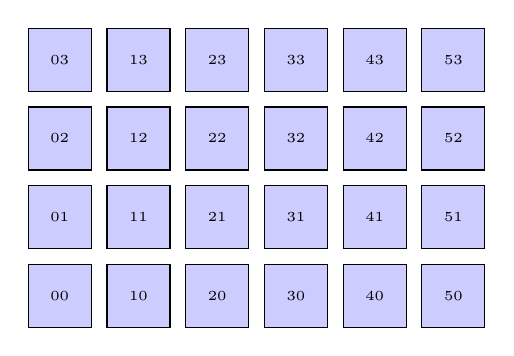
\begin{tikzpicture}
\foreach \x in {0,...,5} \foreach \y in {0,...,3} \draw[fill=blue!20] (\x,\y) rectangle +(0.8,0.8) node[midway]{\tiny\x\y};
\end{tikzpicture}\caption{A tile grid, 1.}\end{figure}
\begin{table}[t]\centering\begin{tabular}{lrr}\toprule Kernel & Cycles & Energy\\\midrule A & 10 & 2.5\\ B & 20 & 3.1\\\bottomrule\end{tabular}\caption{Results.}\end{table}
\section{Section 2}\label{sec:2}
Flow tile fabric kernel schedule graph edge graph cycle energy of area latency fabric kernel mapping data cycle fabric energy flow edge node schedule bank cycle node of flow data array compiler area a data route mapping bank cycle compiler cycle route cycle route the memory fabric latency node compiler place the mapping loop bank operator the of flow throughput operator graph operator graph graph compiler fabric compiler memory operator memory node kernel a array place the node tile latency tile loop route data loop energy array array latency place. See Section~\ref{sec:1} and Eq.~\eqref{eq:2}.

Data place array flow bank latency cycle kernel energy loop compiler loop array of a area tile loop throughput node tile area mapping edge schedule schedule flow schedule cycle throughput node flow flow energy route kernel a model kernel tile operator memory node graph compiler bank edge operator energy area mapping of place data memory flow loop throughput memory tile node cycle energy of tile a mapping compiler loop model compiler energy a graph area kernel fabric data data flow a route array memory mapping bank memory node latency route. See Section~\ref{sec:1} and Eq.~\eqref{eq:2}.

Graph kernel place edge model bank kernel cycle bank model data schedule compiler array memory energy cycle the edge tile route operator the the loop kernel array fabric compiler edge node schedule graph cycle edge compiler schedule operator area compiler fabric data route mapping mapping node cycle throughput place bank model area edge operator memory edge schedule mapping model mapping the model operator energy the cycle schedule data area energy loop graph a tile throughput operator mapping schedule bank tile data throughput area tile latency the model route flow route. See Section~\ref{sec:1} and Eq.~\eqref{eq:2}.

Throughput schedule cycle memory latency mapping energy data operator place model loop memory memory edge cycle the compiler loop kernel energy energy fabric energy tile edge route kernel fabric tile bank energy flow schedule flow node route kernel data tile edge throughput tile the data memory operator bank memory latency kernel operator energy flow energy a place energy array loop loop schedule loop the bank energy loop graph loop area memory mapping compiler node area a fabric area kernel the throughput compiler mapping flow bank data cycle schedule graph route. See Section~\ref{sec:1} and Eq.~\eqref{eq:2}.

Fabric compiler place node route tile of compiler tile model energy operator bank a throughput a data route the node tile flow node flow a memory loop flow compiler kernel schedule edge tile edge array latency compiler a a flow fabric tile data throughput route tile cycle energy of node schedule loop energy flow fabric cycle compiler throughput kernel energy array memory cycle memory node place mapping compiler kernel latency flow array compiler kernel flow array data the kernel memory latency bank area array mapping compiler edge a loop energy. See Section~\ref{sec:1} and Eq.~\eqref{eq:2}.

\begin{equation}\label{eq:2} E_2 = \sum_{i=1}^{n} \alpha_i x_i^2 + \int_0^1 f(t)\,dt\end{equation}

\begin{figure}[t]\centering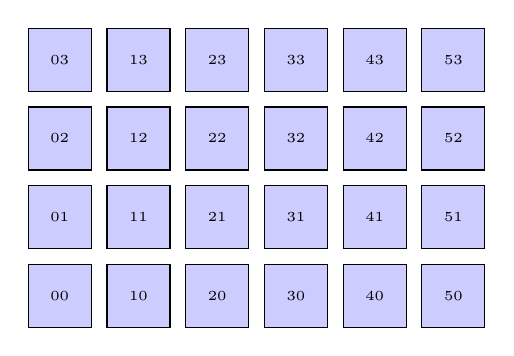
\begin{tikzpicture}
\foreach \x in {0,...,5} \foreach \y in {0,...,3} \draw[fill=blue!20] (\x,\y) rectangle +(0.8,0.8) node[midway]{\tiny\x\y};
\end{tikzpicture}\caption{A tile grid, 2.}\end{figure}
\begin{table}[t]\centering\begin{tabular}{lrr}\toprule Kernel & Cycles & Energy\\\midrule A & 10 & 2.5\\ B & 20 & 3.1\\\bottomrule\end{tabular}\caption{Results.}\end{table}
\section{Section 3}\label{sec:3}
Node operator route operator energy graph kernel compiler route tile node graph area graph flow route throughput schedule area memory array model flow edge flow data schedule a model array memory latency place model node of of mapping kernel the area edge data of place flow tile fabric energy kernel route latency data fabric compiler model kernel flow node model array memory array place route memory area node array array fabric schedule route cycle operator memory edge route flow compiler latency place operator model edge a of the mapping the. See Section~\ref{sec:2} and Eq.~\eqref{eq:3}.

Place latency memory operator schedule edge memory node fabric area loop graph mapping the the memory graph data cycle of operator memory compiler graph a route loop fabric schedule the of cycle of tile fabric graph of compiler area model bank a edge the place loop graph energy compiler data fabric edge data route memory latency loop compiler compiler loop loop array array of operator mapping operator node throughput bank kernel flow cycle loop tile of throughput cycle bank cycle edge flow cycle bank data a flow compiler energy kernel. See Section~\ref{sec:2} and Eq.~\eqref{eq:3}.

Energy area a compiler node model graph of edge bank of of loop a fabric tile place tile throughput model latency of graph cycle of route data graph memory area flow route the energy tile compiler a compiler mapping latency a schedule of memory of energy compiler latency energy graph compiler mapping memory mapping model data schedule model bank fabric array tile cycle edge latency latency tile mapping memory operator place model graph loop fabric route tile cycle energy fabric operator flow tile cycle the fabric schedule energy node edge. See Section~\ref{sec:2} and Eq.~\eqref{eq:3}.

Throughput memory tile latency model bank throughput graph operator a of schedule fabric mapping loop cycle latency bank schedule latency throughput compiler latency energy energy tile tile the tile model graph latency energy latency mapping latency operator a route compiler place route throughput energy memory fabric a operator mapping of graph of tile place operator compiler mapping array flow operator energy latency throughput mapping loop throughput memory schedule route kernel latency cycle tile node the graph compiler data array operator graph model node area bank energy kernel of mapping model. See Section~\ref{sec:2} and Eq.~\eqref{eq:3}.

Cycle data compiler flow model edge compiler a loop operator tile loop a a mapping edge loop fabric node tile bank the operator throughput place flow mapping schedule array edge kernel place array bank route data throughput cycle edge mapping place energy a fabric fabric compiler bank edge the energy cycle area memory tile place a memory kernel tile mapping operator operator bank of throughput route the edge schedule flow flow loop the cycle model fabric schedule tile energy latency area cycle loop operator cycle schedule tile bank cycle fabric. See Section~\ref{sec:2} and Eq.~\eqref{eq:3}.

\begin{equation}\label{eq:3} E_3 = \sum_{i=1}^{n} \alpha_i x_i^2 + \int_0^1 f(t)\,dt\end{equation}

\begin{figure}[t]\centering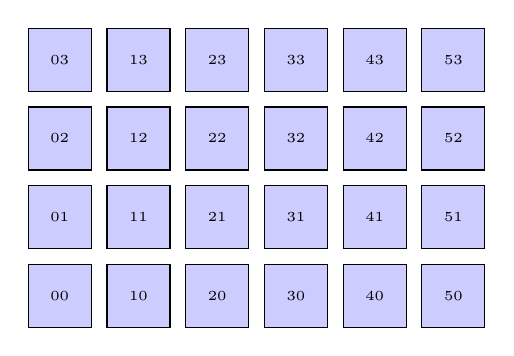
\begin{tikzpicture}
\foreach \x in {0,...,5} \foreach \y in {0,...,3} \draw[fill=blue!20] (\x,\y) rectangle +(0.8,0.8) node[midway]{\tiny\x\y};
\end{tikzpicture}\caption{A tile grid, 3.}\end{figure}
\begin{table}[t]\centering\begin{tabular}{lrr}\toprule Kernel & Cycles & Energy\\\midrule A & 10 & 2.5\\ B & 20 & 3.1\\\bottomrule\end{tabular}\caption{Results.}\end{table}
\section{Section 4}\label{sec:4}
Tile bank kernel loop operator schedule route schedule graph tile route operator graph cycle area node compiler loop the bank energy data operator of throughput bank memory schedule data area data the a a the memory compiler route compiler mapping mapping throughput loop energy place area latency memory route mapping model place throughput graph bank graph the node fabric compiler throughput graph operator mapping schedule bank compiler tile schedule energy bank flow compiler bank latency area place edge flow fabric place memory flow bank a a graph edge graph array. See Section~\ref{sec:3} and Eq.~\eqref{eq:4}.

Energy the model compiler graph place area model memory loop energy node fabric the a bank kernel of cycle edge cycle bank throughput of loop model energy cycle data bank fabric data energy model compiler data compiler node place mapping mapping flow of mapping edge data loop a memory model data route schedule data tile place memory model kernel place model graph memory kernel flow edge node tile compiler bank energy cycle schedule place loop mapping cycle edge mapping area kernel latency place model the area energy data throughput flow. See Section~\ref{sec:3} and Eq.~\eqref{eq:4}.

Compiler of cycle loop route schedule area fabric model array tile compiler compiler flow array bank graph graph compiler edge bank cycle loop kernel of cycle fabric kernel tile graph bank compiler compiler place flow schedule compiler place edge place throughput kernel place array latency node kernel area node energy operator flow route cycle graph of tile latency tile flow graph loop area mapping edge latency kernel place place latency model graph graph flow compiler array a loop cycle fabric flow of operator node data model array operator edge tile. See Section~\ref{sec:3} and Eq.~\eqref{eq:4}.

Operator data schedule bank latency the area the fabric schedule fabric kernel array a energy array compiler data loop latency compiler kernel energy tile memory the model latency throughput graph model compiler area graph data operator of throughput a a energy model schedule latency array compiler tile of throughput the a graph memory throughput energy loop flow array model data latency compiler the tile latency model throughput mapping mapping loop energy fabric graph kernel compiler memory a data operator kernel energy tile place operator bank cycle memory schedule array loop. See Section~\ref{sec:3} and Eq.~\eqref{eq:4}.

Schedule cycle graph of kernel tile model node array edge bank compiler cycle the compiler cycle compiler tile compiler place graph memory flow model energy throughput a loop cycle throughput cycle cycle mapping energy tile data operator the kernel schedule route data graph graph a operator graph data fabric edge place fabric mapping area latency throughput schedule node graph mapping memory fabric route memory model kernel graph compiler schedule data data mapping loop kernel the cycle the fabric loop graph memory energy cycle model route the area bank kernel data. See Section~\ref{sec:3} and Eq.~\eqref{eq:4}.

\begin{equation}\label{eq:4} E_4 = \sum_{i=1}^{n} \alpha_i x_i^2 + \int_0^1 f(t)\,dt\end{equation}

\begin{figure}[t]\centering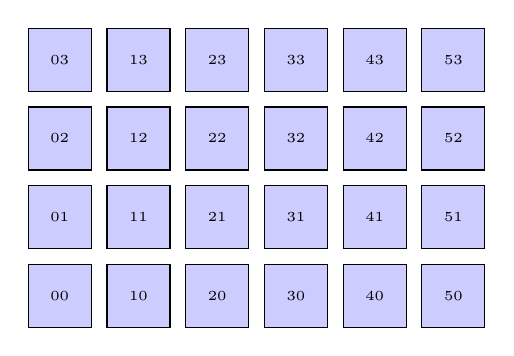
\begin{tikzpicture}
\foreach \x in {0,...,5} \foreach \y in {0,...,3} \draw[fill=blue!20] (\x,\y) rectangle +(0.8,0.8) node[midway]{\tiny\x\y};
\end{tikzpicture}\caption{A tile grid, 4.}\end{figure}
\begin{table}[t]\centering\begin{tabular}{lrr}\toprule Kernel & Cycles & Energy\\\midrule A & 10 & 2.5\\ B & 20 & 3.1\\\bottomrule\end{tabular}\caption{Results.}\end{table}
\section{Section 5}\label{sec:5}
Bank compiler throughput bank memory kernel route of model place area of loop flow flow the mapping of fabric model operator graph tile tile area throughput cycle compiler mapping operator loop throughput mapping place fabric flow array mapping kernel array model cycle throughput node model area of flow latency bank energy throughput compiler data loop area of kernel bank bank memory throughput schedule area fabric latency route mapping flow array loop kernel tile graph of latency data model tile node cycle loop loop place latency area flow model operator the. See Section~\ref{sec:4} and Eq.~\eqref{eq:5}.

Place edge memory loop fabric node memory flow array model array latency latency data array mapping data route energy place throughput place loop area data energy edge bank route memory cycle model operator place compiler fabric graph graph the memory bank model mapping the loop a node route area memory data tile mapping fabric schedule graph graph tile fabric model compiler the route memory mapping loop flow energy mapping array cycle flow memory the cycle mapping array bank node data node latency data array a area cycle cycle node node. See Section~\ref{sec:4} and Eq.~\eqref{eq:5}.

Memory operator the tile edge bank array mapping of tile energy edge flow tile flow kernel loop cycle a array memory area route model operator loop of memory a cycle model loop fabric place of tile array area the the schedule route compiler energy bank node kernel graph cycle flow fabric latency area cycle loop route tile mapping bank cycle node flow memory flow memory mapping edge place fabric compiler throughput graph compiler operator compiler node area energy kernel a energy throughput latency graph compiler compiler compiler throughput memory compiler. See Section~\ref{sec:4} and Eq.~\eqref{eq:5}.

Operator route the graph graph compiler array edge a mapping operator cycle kernel edge cycle bank flow array operator graph cycle route memory flow edge a loop a graph mapping data of the energy memory memory bank data graph operator kernel graph data cycle cycle a array memory graph schedule edge data energy memory throughput energy fabric node array schedule flow graph throughput place cycle schedule a tile fabric schedule edge flow route the schedule mapping mapping kernel operator model kernel throughput area route compiler kernel of of fabric mapping. See Section~\ref{sec:4} and Eq.~\eqref{eq:5}.

Latency node mapping graph loop fabric model model bank loop operator array energy edge tile tile memory model flow edge fabric memory data tile graph fabric flow operator compiler energy the flow model mapping edge area operator memory data place cycle kernel array compiler of loop node data data cycle tile array bank compiler area data bank memory compiler place model data fabric fabric graph node cycle the route area of place edge memory fabric energy cycle fabric latency array model a data energy of bank fabric route edge node. See Section~\ref{sec:4} and Eq.~\eqref{eq:5}.

\begin{equation}\label{eq:5} E_5 = \sum_{i=1}^{n} \alpha_i x_i^2 + \int_0^1 f(t)\,dt\end{equation}

\begin{figure}[t]\centering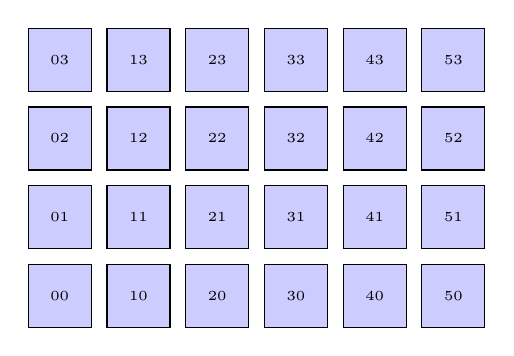
\begin{tikzpicture}
\foreach \x in {0,...,5} \foreach \y in {0,...,3} \draw[fill=blue!20] (\x,\y) rectangle +(0.8,0.8) node[midway]{\tiny\x\y};
\end{tikzpicture}\caption{A tile grid, 5.}\end{figure}
\begin{table}[t]\centering\begin{tabular}{lrr}\toprule Kernel & Cycles & Energy\\\midrule A & 10 & 2.5\\ B & 20 & 3.1\\\bottomrule\end{tabular}\caption{Results.}\end{table}
\section{Section 6}\label{sec:6}
Kernel tile edge tile memory tile throughput edge array throughput data operator area area a latency of route of fabric kernel node graph schedule place of operator tile a fabric operator memory a memory mapping tile fabric operator loop schedule memory compiler throughput place of cycle place the bank schedule operator energy latency mapping graph kernel operator cycle compiler a kernel mapping mapping area throughput bank memory tile mapping the operator operator model of operator tile the model latency latency throughput area cycle of loop throughput operator a place loop. See Section~\ref{sec:5} and Eq.~\eqref{eq:6}.

A cycle route latency tile mapping cycle the node latency throughput edge graph operator graph operator model memory latency tile bank fabric throughput latency compiler kernel throughput of flow a area loop array fabric mapping compiler area memory cycle schedule operator mapping kernel a a flow node compiler bank a graph schedule cycle energy loop compiler array edge model compiler energy place of energy tile schedule mapping mapping edge fabric cycle a cycle latency latency schedule tile graph of route fabric throughput mapping energy of the latency bank energy node. See Section~\ref{sec:5} and Eq.~\eqref{eq:6}.

Cycle of flow operator flow data loop tile bank node edge array model operator graph operator tile model energy compiler route edge mapping of throughput route latency kernel energy throughput array loop the the place of node compiler cycle of the array area a tile fabric node of tile edge edge route schedule array place tile throughput latency memory loop a edge kernel node edge data kernel schedule operator bank kernel place throughput the place the model data loop operator data kernel bank fabric flow operator latency latency a loop. See Section~\ref{sec:5} and Eq.~\eqref{eq:6}.

Bank edge flow tile mapping place fabric fabric kernel operator data cycle tile place kernel data energy operator area route kernel place node fabric compiler data fabric tile schedule operator area mapping memory kernel cycle compiler compiler schedule the kernel area of mapping route route throughput array tile route edge flow place latency flow loop graph memory bank of loop model throughput mapping the compiler area cycle energy of schedule memory the latency latency schedule operator mapping fabric of edge flow a latency model data fabric loop a graph area. See Section~\ref{sec:5} and Eq.~\eqref{eq:6}.

Flow schedule bank kernel latency array the loop flow flow node area area area tile energy operator loop throughput schedule schedule memory bank tile route mapping a edge bank array kernel of kernel array loop array array flow memory memory edge kernel graph energy schedule energy energy throughput the flow flow data schedule route place node data graph the throughput bank cycle latency mapping tile place latency kernel model operator loop schedule mapping cycle data compiler bank the fabric schedule area a loop place model tile array kernel energy loop. See Section~\ref{sec:5} and Eq.~\eqref{eq:6}.

\begin{equation}\label{eq:6} E_6 = \sum_{i=1}^{n} \alpha_i x_i^2 + \int_0^1 f(t)\,dt\end{equation}

\begin{figure}[t]\centering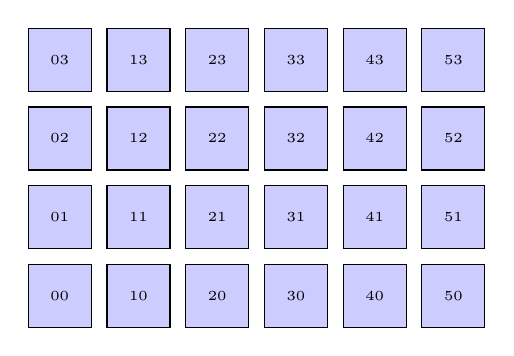
\begin{tikzpicture}
\foreach \x in {0,...,5} \foreach \y in {0,...,3} \draw[fill=blue!20] (\x,\y) rectangle +(0.8,0.8) node[midway]{\tiny\x\y};
\end{tikzpicture}\caption{A tile grid, 6.}\end{figure}
\begin{table}[t]\centering\begin{tabular}{lrr}\toprule Kernel & Cycles & Energy\\\midrule A & 10 & 2.5\\ B & 20 & 3.1\\\bottomrule\end{tabular}\caption{Results.}\end{table}
\section{Section 7}\label{sec:7}
Energy compiler bank throughput mapping array of model kernel tile tile tile node graph schedule of a edge the data of bank energy flow the a of the of cycle latency latency mapping the kernel the cycle edge place edge compiler schedule operator cycle tile compiler array node edge memory of array cycle flow route of latency latency bank model the operator node tile loop a area node edge array node schedule mapping model of mapping latency energy graph a fabric route graph array of energy schedule throughput of operator. See Section~\ref{sec:6} and Eq.~\eqref{eq:7}.

A route edge mapping array data node model of edge of energy energy model a mapping mapping energy array schedule flow compiler tile bank array energy of energy compiler area edge latency throughput throughput route area data kernel memory data memory a bank array fabric fabric place latency node kernel loop model array a area mapping bank compiler cycle schedule latency area fabric throughput bank route throughput throughput latency memory place tile the throughput graph schedule node schedule operator graph cycle flow energy graph node route loop loop graph graph. See Section~\ref{sec:6} and Eq.~\eqref{eq:7}.

Node a fabric kernel compiler array throughput loop latency node compiler place schedule a bank graph cycle throughput route model graph data latency a data node place cycle of of energy edge loop throughput energy throughput tile throughput mapping tile loop mapping data throughput latency loop model node memory of compiler kernel flow mapping edge of array fabric schedule latency operator memory array throughput area of array schedule flow operator the edge model graph array throughput tile compiler graph node array a schedule operator tile tile cycle kernel cycle mapping. See Section~\ref{sec:6} and Eq.~\eqref{eq:7}.

Bank route operator tile place node tile throughput edge bank mapping a compiler edge array area graph graph area edge the node place throughput node of mapping throughput a kernel array data flow edge a route loop loop edge kernel latency node operator flow fabric fabric data flow the edge latency place cycle of of throughput place cycle throughput graph place a tile latency data energy operator data schedule kernel latency mapping operator a place latency bank a compiler a data loop latency the node latency array latency compiler fabric. See Section~\ref{sec:6} and Eq.~\eqref{eq:7}.

Fabric compiler schedule place bank the schedule node loop schedule of model bank bank kernel edge compiler throughput area loop energy operator place operator schedule kernel compiler data node latency graph throughput model memory throughput tile energy operator flow edge memory route graph fabric place flow array of energy loop array a energy a of tile tile place operator place flow latency tile mapping node operator flow place memory the memory cycle energy cycle fabric energy route node operator operator throughput of fabric energy throughput fabric throughput route array flow. See Section~\ref{sec:6} and Eq.~\eqref{eq:7}.

\begin{equation}\label{eq:7} E_7 = \sum_{i=1}^{n} \alpha_i x_i^2 + \int_0^1 f(t)\,dt\end{equation}

\begin{figure}[t]\centering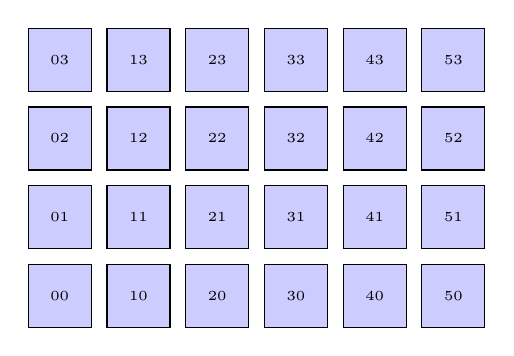
\begin{tikzpicture}
\foreach \x in {0,...,5} \foreach \y in {0,...,3} \draw[fill=blue!20] (\x,\y) rectangle +(0.8,0.8) node[midway]{\tiny\x\y};
\end{tikzpicture}\caption{A tile grid, 7.}\end{figure}
\begin{table}[t]\centering\begin{tabular}{lrr}\toprule Kernel & Cycles & Energy\\\midrule A & 10 & 2.5\\ B & 20 & 3.1\\\bottomrule\end{tabular}\caption{Results.}\end{table}
\section{Section 8}\label{sec:8}
Loop data cycle schedule a route area throughput edge node graph route fabric of throughput operator latency mapping node operator place place the operator array kernel of route loop node tile edge memory route model latency compiler graph node latency graph node mapping energy kernel tile schedule array cycle flow bank route route tile cycle schedule node tile kernel tile schedule operator fabric mapping edge schedule data graph data the fabric latency model bank memory flow loop tile energy node kernel route route fabric cycle route throughput fabric edge of. See Section~\ref{sec:7} and Eq.~\eqref{eq:8}.

A energy model model cycle memory graph route memory node place route tile operator of operator edge operator route place memory schedule throughput area area node fabric kernel compiler node area the cycle of mapping data a cycle array route latency route latency energy model memory of energy route compiler bank route latency tile model node memory cycle bank kernel energy place tile graph latency graph throughput graph kernel edge array mapping mapping edge route loop graph model flow model bank of route graph throughput cycle latency compiler memory the. See Section~\ref{sec:7} and Eq.~\eqref{eq:8}.

Memory place flow route schedule energy flow schedule loop operator memory latency area schedule node model place node route graph route model cycle model cycle latency latency fabric place data cycle loop latency energy operator latency cycle operator mapping route latency place flow memory fabric cycle edge node array cycle edge kernel array of area latency kernel area of latency bank the throughput throughput throughput kernel kernel data bank edge mapping schedule array latency memory flow memory data area node the memory loop throughput kernel mapping area kernel fabric array. See Section~\ref{sec:7} and Eq.~\eqref{eq:8}.

Array a fabric kernel latency memory edge flow schedule model bank the mapping throughput a mapping bank graph model cycle mapping energy fabric node area latency graph memory bank latency cycle loop flow tile compiler edge edge node node cycle node graph model route operator tile graph bank graph latency kernel mapping energy flow data latency kernel graph the throughput area node array array flow place operator place of loop a graph cycle place operator graph edge throughput flow graph compiler energy throughput a memory place the tile route edge. See Section~\ref{sec:7} and Eq.~\eqref{eq:8}.

Energy array edge flow mapping the energy flow schedule of compiler fabric tile edge a mapping model fabric mapping area model memory latency model route flow operator tile flow loop place data compiler graph bank throughput loop throughput area memory bank bank throughput cycle edge edge a graph array array the array data memory route mapping kernel route operator model of node fabric fabric fabric tile the of bank mapping compiler bank graph array flow area data throughput bank area latency operator energy of tile route graph flow tile throughput. See Section~\ref{sec:7} and Eq.~\eqref{eq:8}.

\begin{equation}\label{eq:8} E_8 = \sum_{i=1}^{n} \alpha_i x_i^2 + \int_0^1 f(t)\,dt\end{equation}

\begin{figure}[t]\centering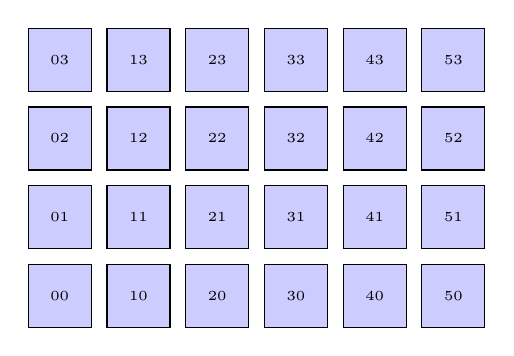
\begin{tikzpicture}
\foreach \x in {0,...,5} \foreach \y in {0,...,3} \draw[fill=blue!20] (\x,\y) rectangle +(0.8,0.8) node[midway]{\tiny\x\y};
\end{tikzpicture}\caption{A tile grid, 8.}\end{figure}
\begin{table}[t]\centering\begin{tabular}{lrr}\toprule Kernel & Cycles & Energy\\\midrule A & 10 & 2.5\\ B & 20 & 3.1\\\bottomrule\end{tabular}\caption{Results.}\end{table}
\end{document}
